\begin{frame}
\frametitle{Marco teórico}

\begin{itemize}
	\item Un \textbf{grafo} $G = (V, E)$ como el conjunto finito de \textit{vértices} $V$ (nodos) y el conjunto de \textit{aristas} $E \subseteq V \times V$ (arcos).
	\item Dos vértices $v_{1}$ y $v_{2} \in V(G)$ son \textbf{adyacentes} o \textbf{vecinos} si $(v_{1}, v_{2}) \in E(G)$ y $v_{1} \neq v_{2}$.
	\item Un grafo es \textbf{no dirigido} cuando la arista conlleva ambos sentidos, es decir $(v_{1}, v_{2}) = (v_{2}, v_{1})$.
	\item El \textbf{grado de un vértice} $d(v)$ es la cantidad de vértices en $V(G)$ que son adyacentes con $v$.
	\item La \textbf{matriz de adyacencia} de un grafo $G$ corresponde a una matriz binaria cuadrada $|V(G)| \times |V(G)|$ donde cada bit representa si un par de vértices $v_{1}$ y $v_{2} \in V(G)$ son vecinos o no.
\end{itemize}

\end{frame}



\begin{frame}
\frametitle{Marco teórico (2)}

\begin{itemize}
	\item Un grafo \textbf{k-degenerate} es no dirigido, donde cada subgrafo tiene un vértice con grado a lo más \textbf{k}. 
	\item El índice de \textbf{degeneracy} de un grafo, $D(G)$, es el menor valor \textbf{k} para el cual el grafo es \textbf{k-degenerate}.
	\item Un \textbf{clique} es un subgrafo donde todos los vértices son adyacentes entre sí. Un \textbf{clique maximal} no es subconjunto de otro clique más grande.
	\begin{figure}
    	\centering
    	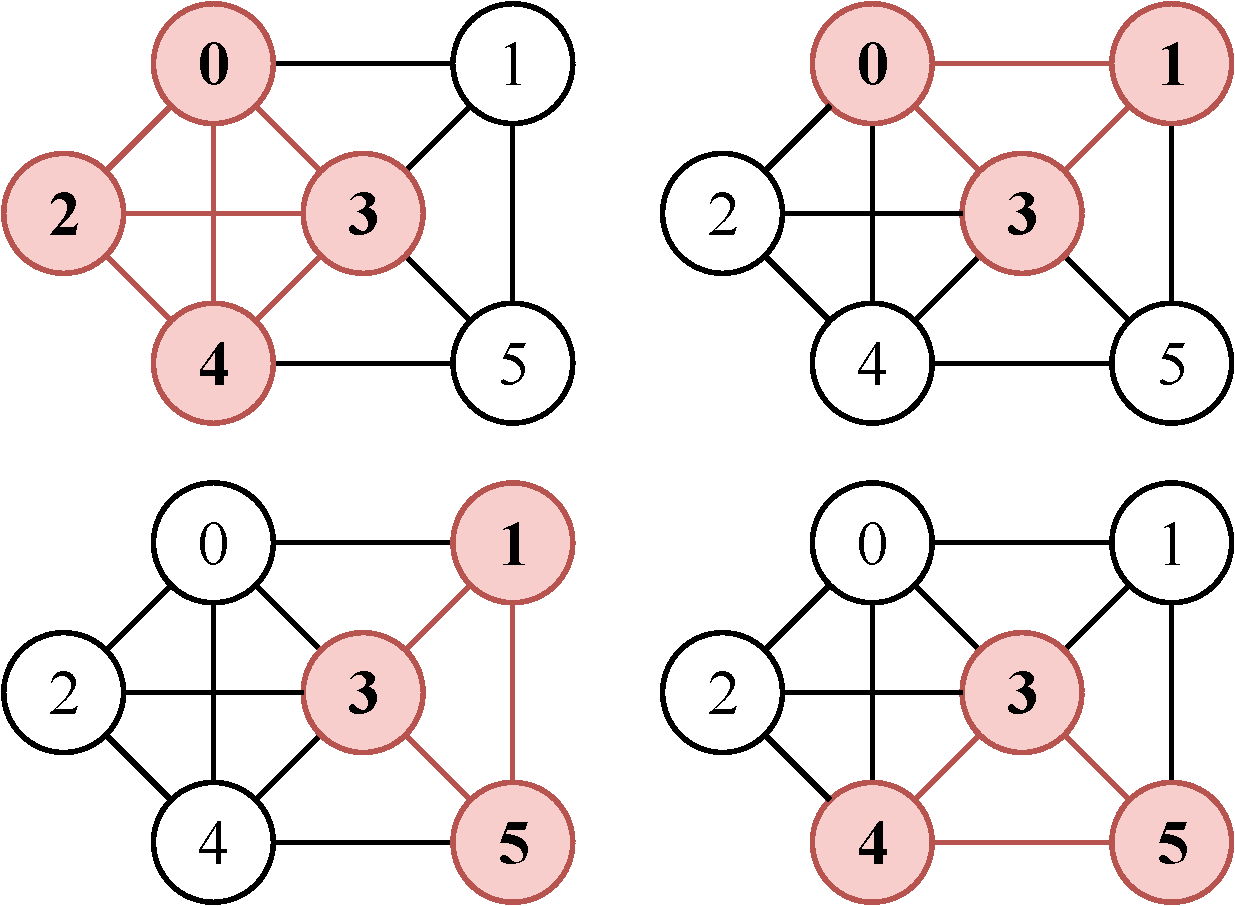
\includegraphics[width=0.4\linewidth]{../img/maxCliqueExample.pdf}
    	
    \caption{Ejemplo de grafo y sus cliques maximales.}
    \label{fig:maxCliqueExample}
\end{figure}
\end{itemize}

\end{frame}


\begin{frame}
\frametitle{Marco teórico (3)}

\begin{itemize}
	\item Un \textbf{triángulo} es un subgrafo de tres vértices y tres aristas. Se define $\lambda(v)$ como la cantidad de triángulos donde participa un nodo $v$.
	\item Se define $\lambda(G)$ como la cantidad de triángulos de un grafo. Se calcula sumando $\lambda(v)$ para cada vértice $v$, y dividiendo el total en tres.
	\begin{equation}
		\lambda(G) = \dfrac{1}{3} \sum_{v \in V} \lambda(v) \label{eq:triangles}
	\end{equation}
	
	\item Un \textbf{triplete} es un subgrafo de tres vértices y dos aristas, donde las aristas comparten un vértice común. Se define $\tau(v)$ como la cantidad de tripletes donde $v$ es el vértice común.
	\item Se define $\tau(G)$ como la cantidad de tripletes de un grafo.
	\begin{equation}
		\tau(G) = \sum_{v \in V} \tau(v) \label{eq:triplets}
	\end{equation}
\end{itemize}

\end{frame}

\begin{frame}
\frametitle{Marco teórico (4)}

\begin{itemize}
	\item El \textbf{coeficiente de clusterización} de un vértice indica cuánto está conectado con sus vecinos, y se define como $c(v) =  \lambda(v) / \tau(v)$. 
	\item El coeficiente de clusterización de un grafo ($C(G)$) es el promedio del coeficiente de todos los nodos del grafo.
	\begin{equation}
		C(G) = \dfrac{1}{|V'|} \sum_{v \in V'} c(v)\label{eq:CC}
	\end{equation}
	con $V' = \{ v \in V | d(v) \geq 2 \}$.
	
	\item La \textbf{transitividad} de un grafo ($T(G)$) es la probabilidad que un par de nodos adyacentes estén interconectados.
	\begin{equation}
		T(G) = \dfrac{3 \lambda(G)}{\tau(G)} \label{eq:T} 
	\end{equation}
\end{itemize}

\end{frame}
